\documentclass[border=10pt, tikz]{standalone}
\usepackage{tikz}
\usetikzlibrary{shapes.geometric, arrows.meta, positioning, calc, backgrounds, fit, decorations.pathreplacing}

\begin{document}

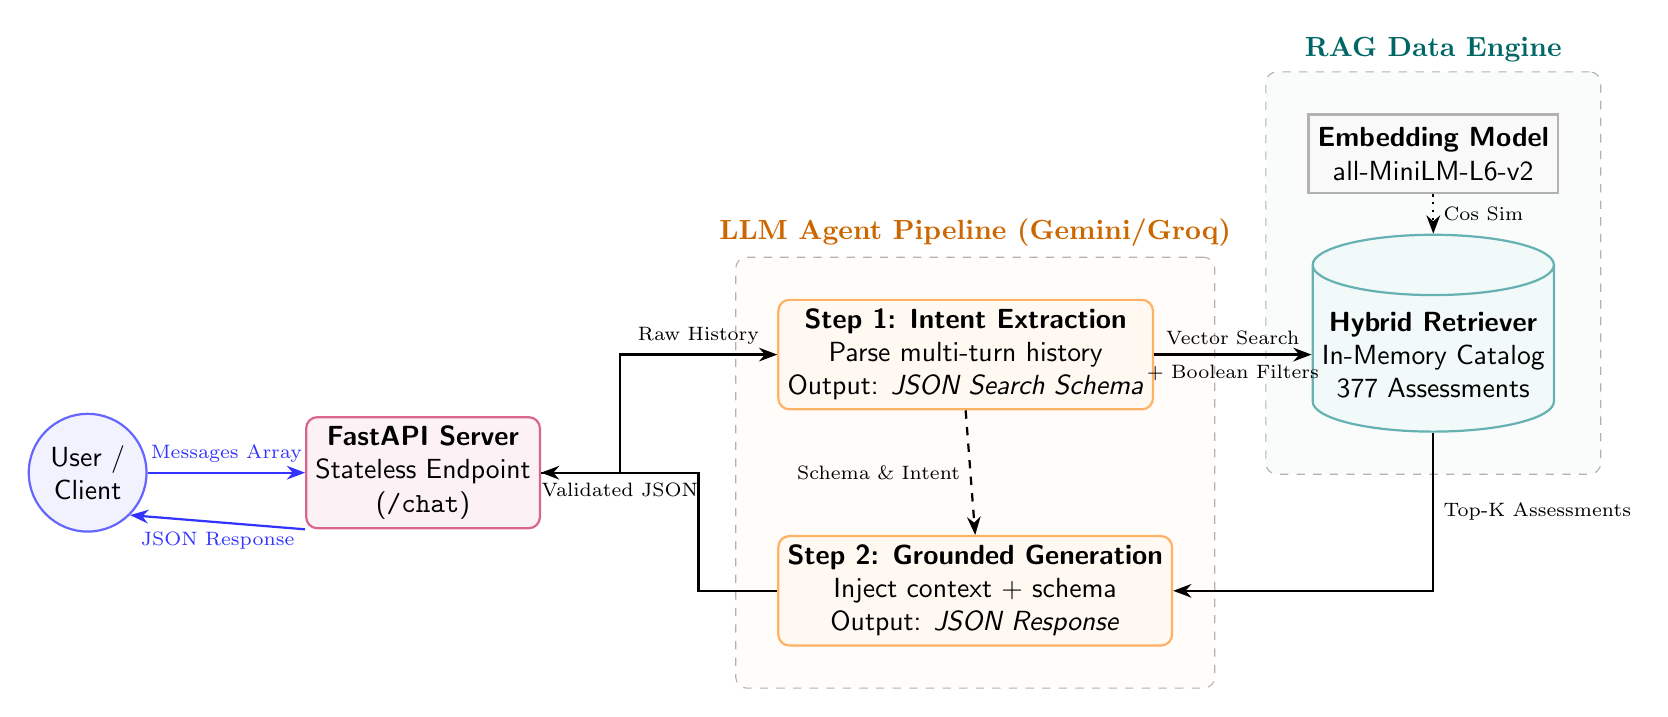
\begin{tikzpicture}[
    font=\sffamily,
    >=Stealth,
    node distance=1.5cm and 2cm,
    % Define styles
    user/.style={circle, draw=blue!60, fill=blue!5, thick, minimum size=1.2cm, align=center},
    api/.style={rectangle, rounded corners, draw=purple!60, fill=purple!5, thick, minimum width=2.5cm, minimum height=1cm, align=center},
    pipeline/.style={rectangle, rounded corners, draw=orange!60, fill=orange!5, thick, minimum width=3.5cm, minimum height=1cm, align=center},
    db/.style={cylinder, shape border rotate=90, aspect=0.25, draw=teal!60, fill=teal!5, thick, minimum width=2.5cm, minimum height=2.5cm, align=center},
    model/.style={rectangle, draw=gray!60, fill=gray!5, thick, minimum width=2.5cm, minimum height=1cm, align=center},
    group/.style={rectangle, rounded corners, draw=black!30, dashed, inner sep=15pt}
]

% 1. User and API
\node[user] (client) {User /\\Client};
\node[api, right=of client] (fastapi) {\textbf{FastAPI Server}\\Stateless Endpoint\\(\texttt{/chat})};

% 2. Agent Pipeline (Two Steps)
\node[pipeline, right=3cm of fastapi, yshift=1.5cm] (intent) {\textbf{Step 1: Intent Extraction}\\Parse multi-turn history\\Output: \textit{JSON Search Schema}};
\node[pipeline, right=3cm of fastapi, yshift=-1.5cm] (generation) {\textbf{Step 2: Grounded Generation}\\Inject context + schema\\Output: \textit{JSON Response}};

% Agent Box
\begin{scope}[on background layer]
    \node[group, fill=orange!2, fit=(intent) (generation)] (agent_box) {};
    \node[above, font=\bfseries, text=orange!80!black] at (agent_box.north) {LLM Agent Pipeline (Gemini/Groq)};
\end{scope}

% 3. Retriever and Data
\node[db, right=2cm of intent] (hybrid) {\textbf{Hybrid Retriever}\\In-Memory Catalog\\377 Assessments};
\node[model, above=0.5cm of hybrid] (embeddings) {\textbf{Embedding Model}\\all-MiniLM-L6-v2};

% Retriever Box
\begin{scope}[on background layer]
    \node[group, fill=teal!2, fit=(hybrid) (embeddings)] (retriever_box) {};
    \node[above, font=\bfseries, text=teal!80!black] at (retriever_box.north) {RAG Data Engine};
\end{scope}

% Connections
% Client to API
\draw[->, thick, blue!80] (client) -- node[above, font=\scriptsize] {Messages Array} (fastapi);
\draw[<-, thick, blue!80] (client.south east) -- node[below, font=\scriptsize] {JSON Response} (fastapi.south west);

% API to Agent Step 1
\draw[->, thick] (fastapi.east) -- +(1,0) |- (intent.west) node[near end, above, font=\scriptsize] {Raw History};

% Agent Step 1 to Retriever
\draw[->, thick] (intent.east) -- node[above, font=\scriptsize] {Vector Search} node[below, font=\scriptsize] {+ Boolean Filters} (hybrid.west);

% Retriever to Agent Step 2
\draw[->, thick] (hybrid.south) |- (generation.east) node[near start, right, font=\scriptsize] {Top-K Assessments};

% Internal Pipeline connection
\draw[->, thick, dashed] (intent.south) -- node[left, font=\scriptsize] {Schema \& Intent} (generation.north);

% Agent Step 2 back to API
\draw[->, thick] (generation.west) -- +( -1,0) |- (fastapi.east) node[near end, below, font=\scriptsize] {Validated JSON};

% Embeddings connection
\draw[->, thick, dotted] (embeddings.south) -- node[right, font=\scriptsize] {Cos Sim} (hybrid.north);

\end{tikzpicture}

\end{document}
